\chapter{Результаты исследования}

На рисунках \ref{img:1}-\ref{img:3} представлен процесс распространения влияния трёх самых влиятельных узлов в десятом по величине сообществе.

\begin{figure}
	\begin{center}
		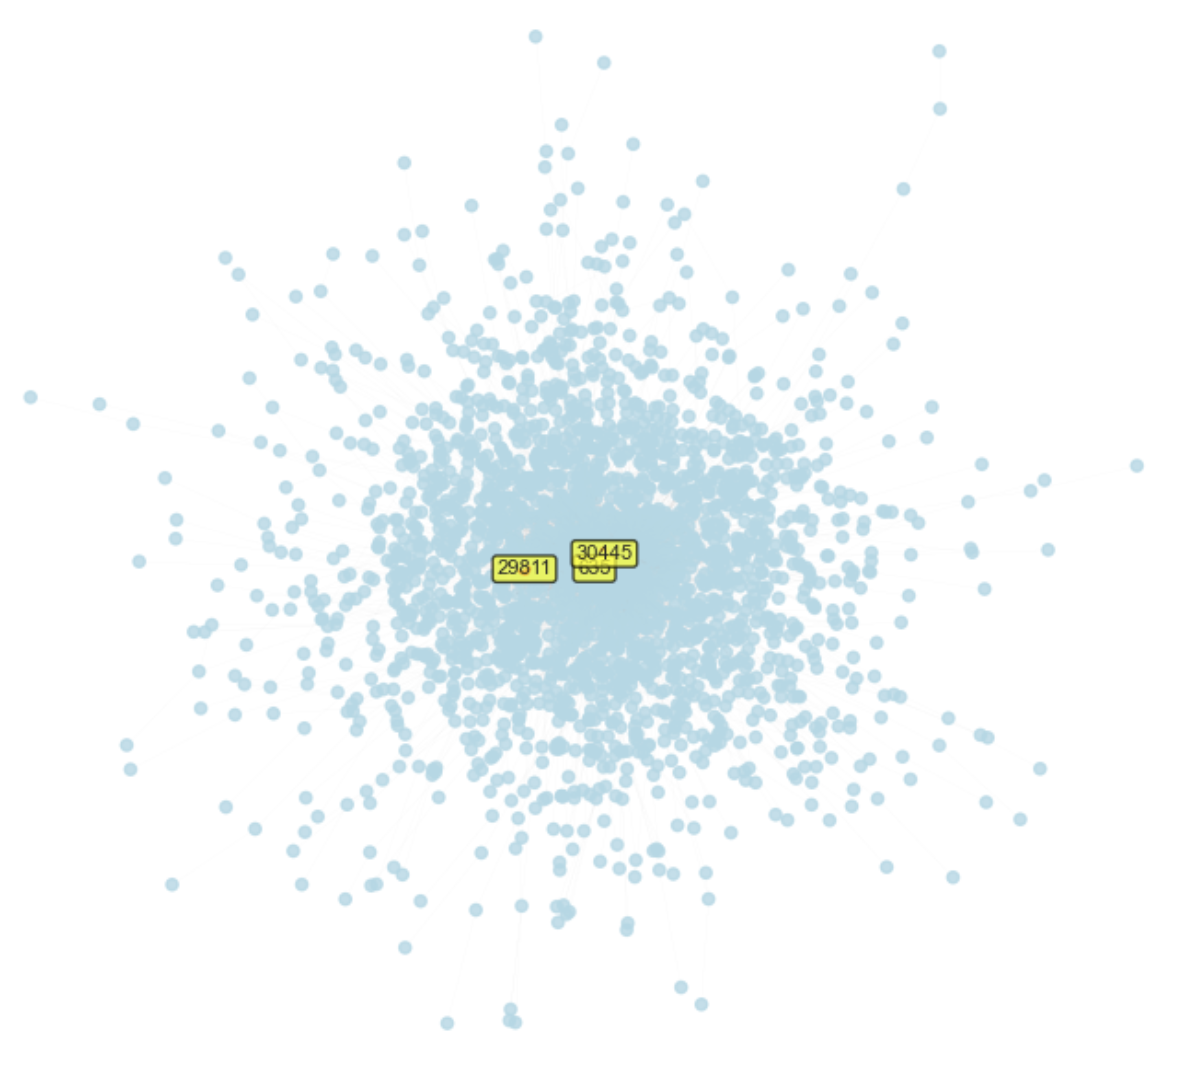
\includegraphics[width=\textwidth]{images/1.png}
	\end{center}
	\caption{Процесс распространения влияния в десятом по величине сообществе (2 382 узла), итерация 0 (только лидеры сообществ)}
	\label{img:1}
\end{figure}

\begin{figure}
	\begin{center}
		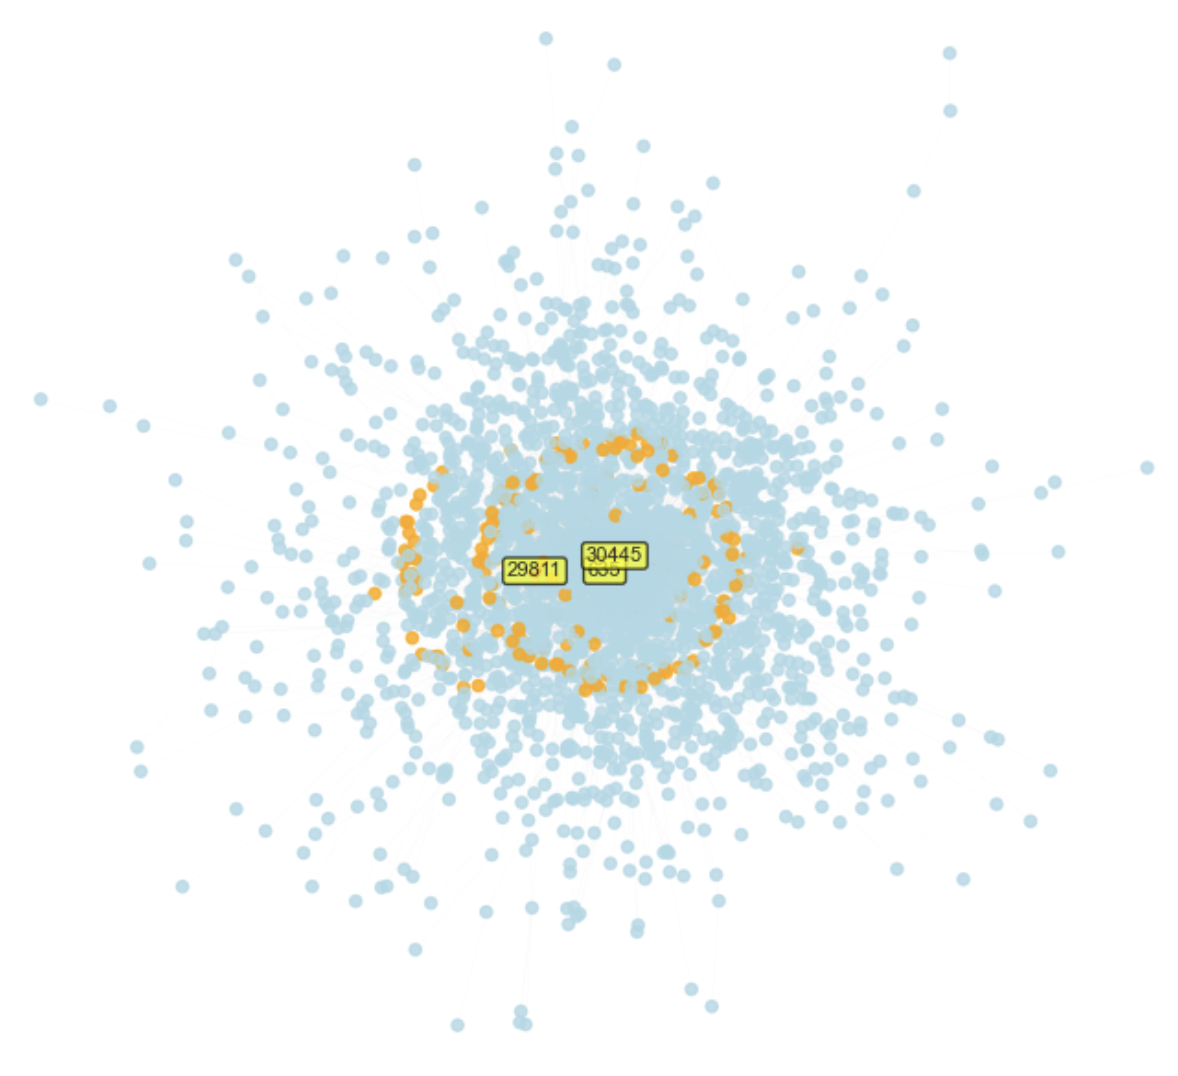
\includegraphics[width=\textwidth]{images/2.png}
	\end{center}
	\caption{Процесс распространения влияния в десятом по величине сообществе (2 382 узла), итерация 1}
	\label{img:2}
\end{figure}

\begin{figure}
	\begin{center}
		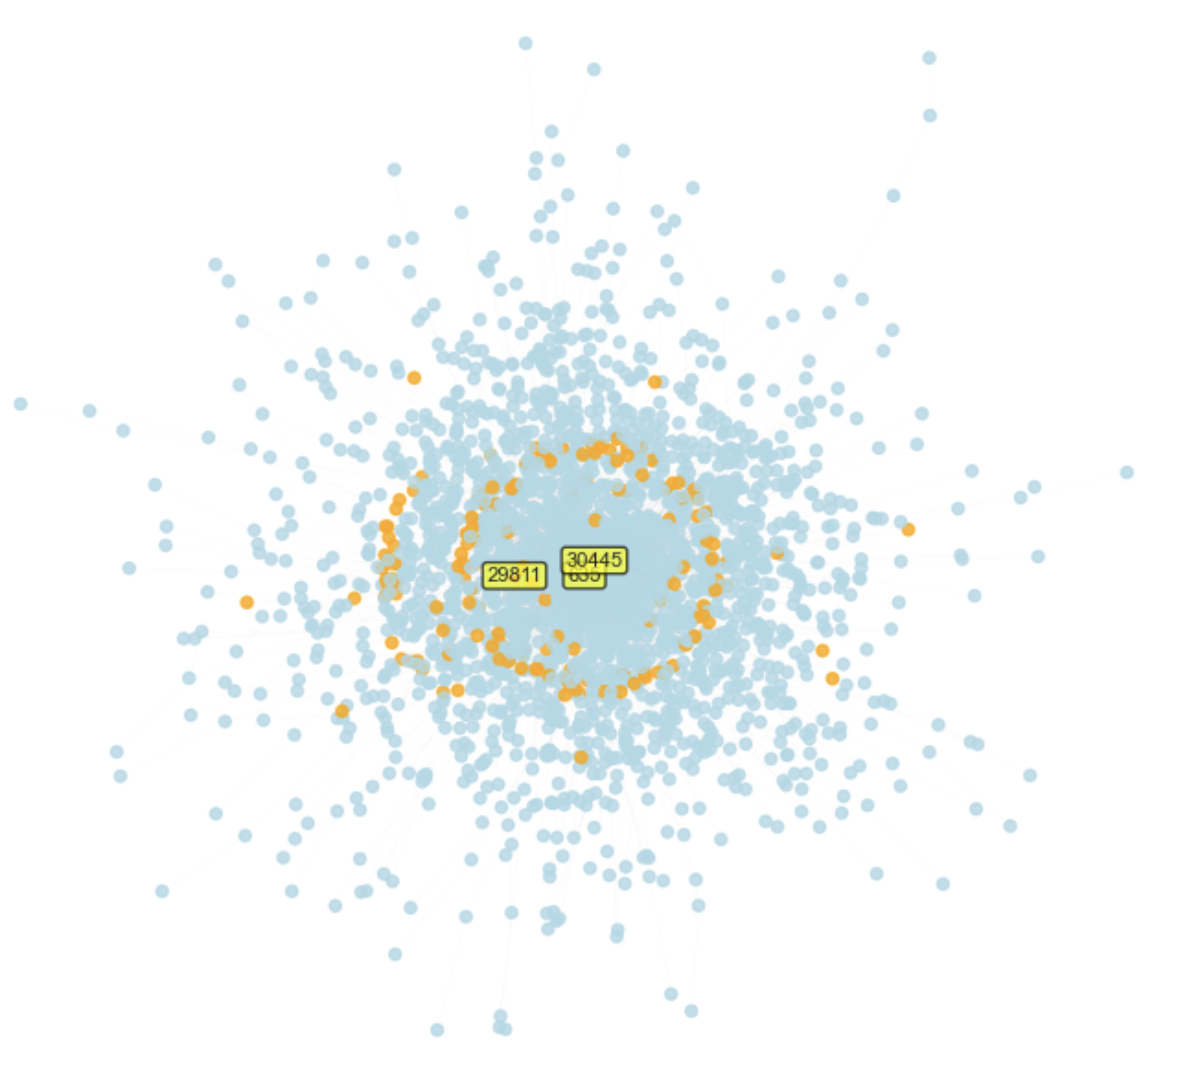
\includegraphics[width=\textwidth]{images/3.png}
	\end{center}
	\caption{Процесс распространения влияния в десятом по величине сообществе (2 382 узла), итерация 2}
	\label{img:3}
\end{figure}

На рисунках \ref{img:4}-\ref{img:6} представлена визуализация 10, 9 и 8 по величине сообществ, положение самых влиятельных узлов выделено зелёным цветом.

\begin{figure}
	\begin{center}
		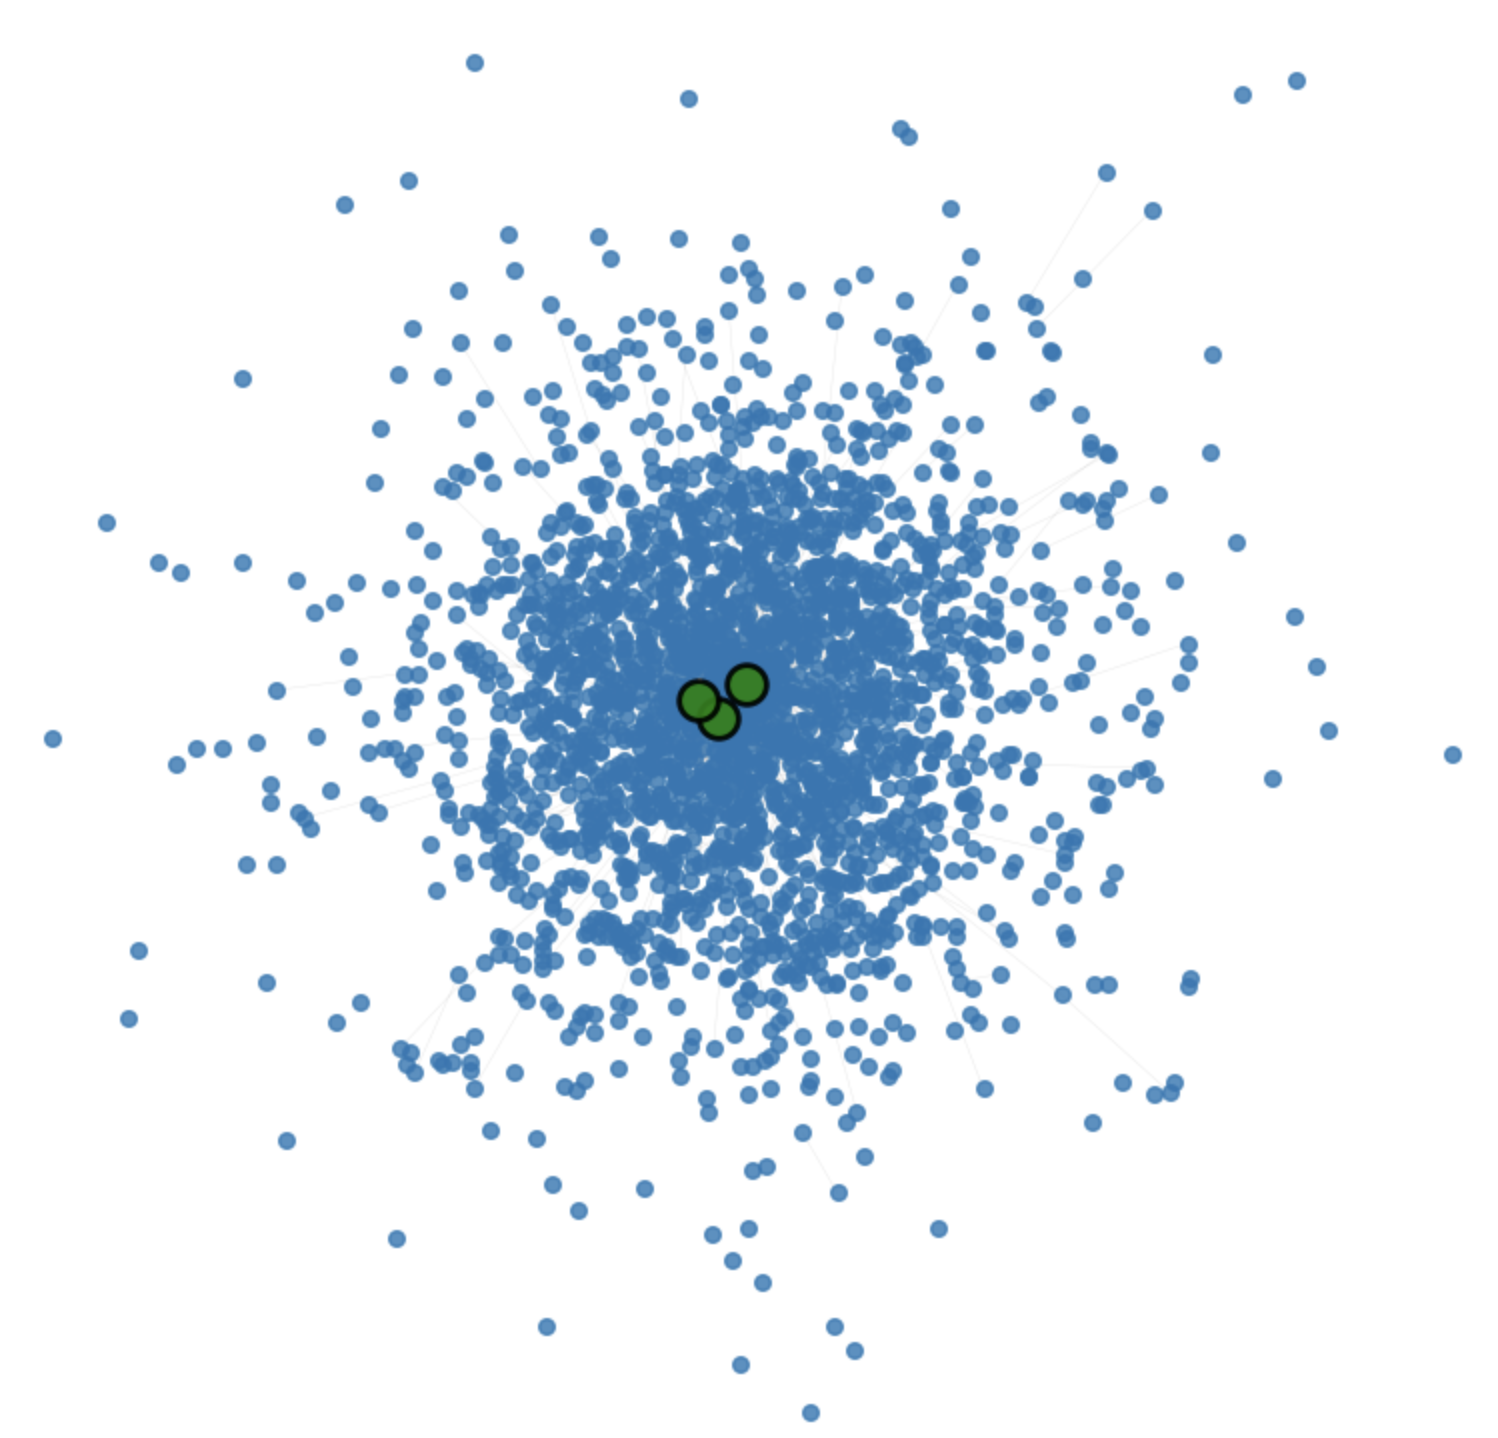
\includegraphics[width=\textwidth]{images/4.png}
	\end{center}
	\caption{Визуализация десятого по величине сообщества (2 382 узла) и трёх самых влиятельных узлов в нём (влияют на 7.0\% сообщества)}
	\label{img:4}
\end{figure}

\begin{figure}
	\begin{center}
		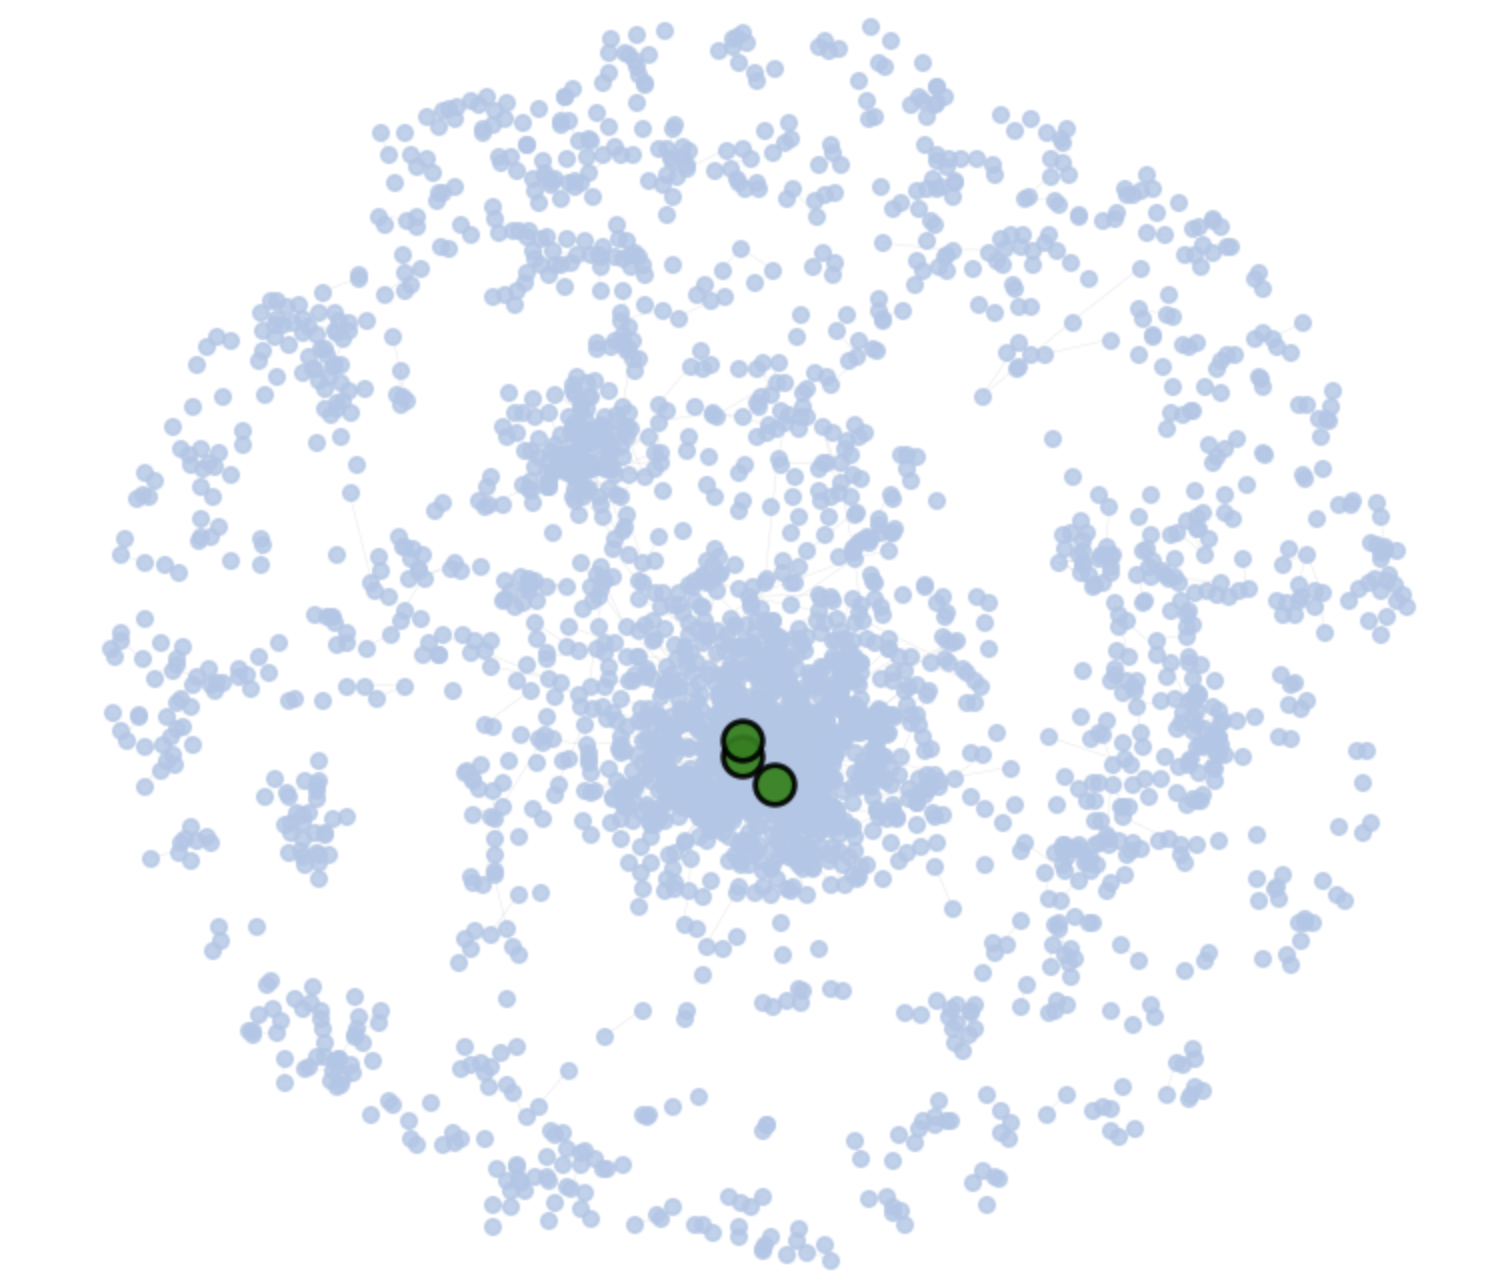
\includegraphics[width=\textwidth]{images/5.png}
	\end{center}
	\caption{Визуализация девятого по величине сообщества (2 700 узлов) и трёх самых влиятельных узлов в нём (влияют на 3.4\% сообщества)}
	\label{img:5}
\end{figure}

\begin{figure}
	\begin{center}
		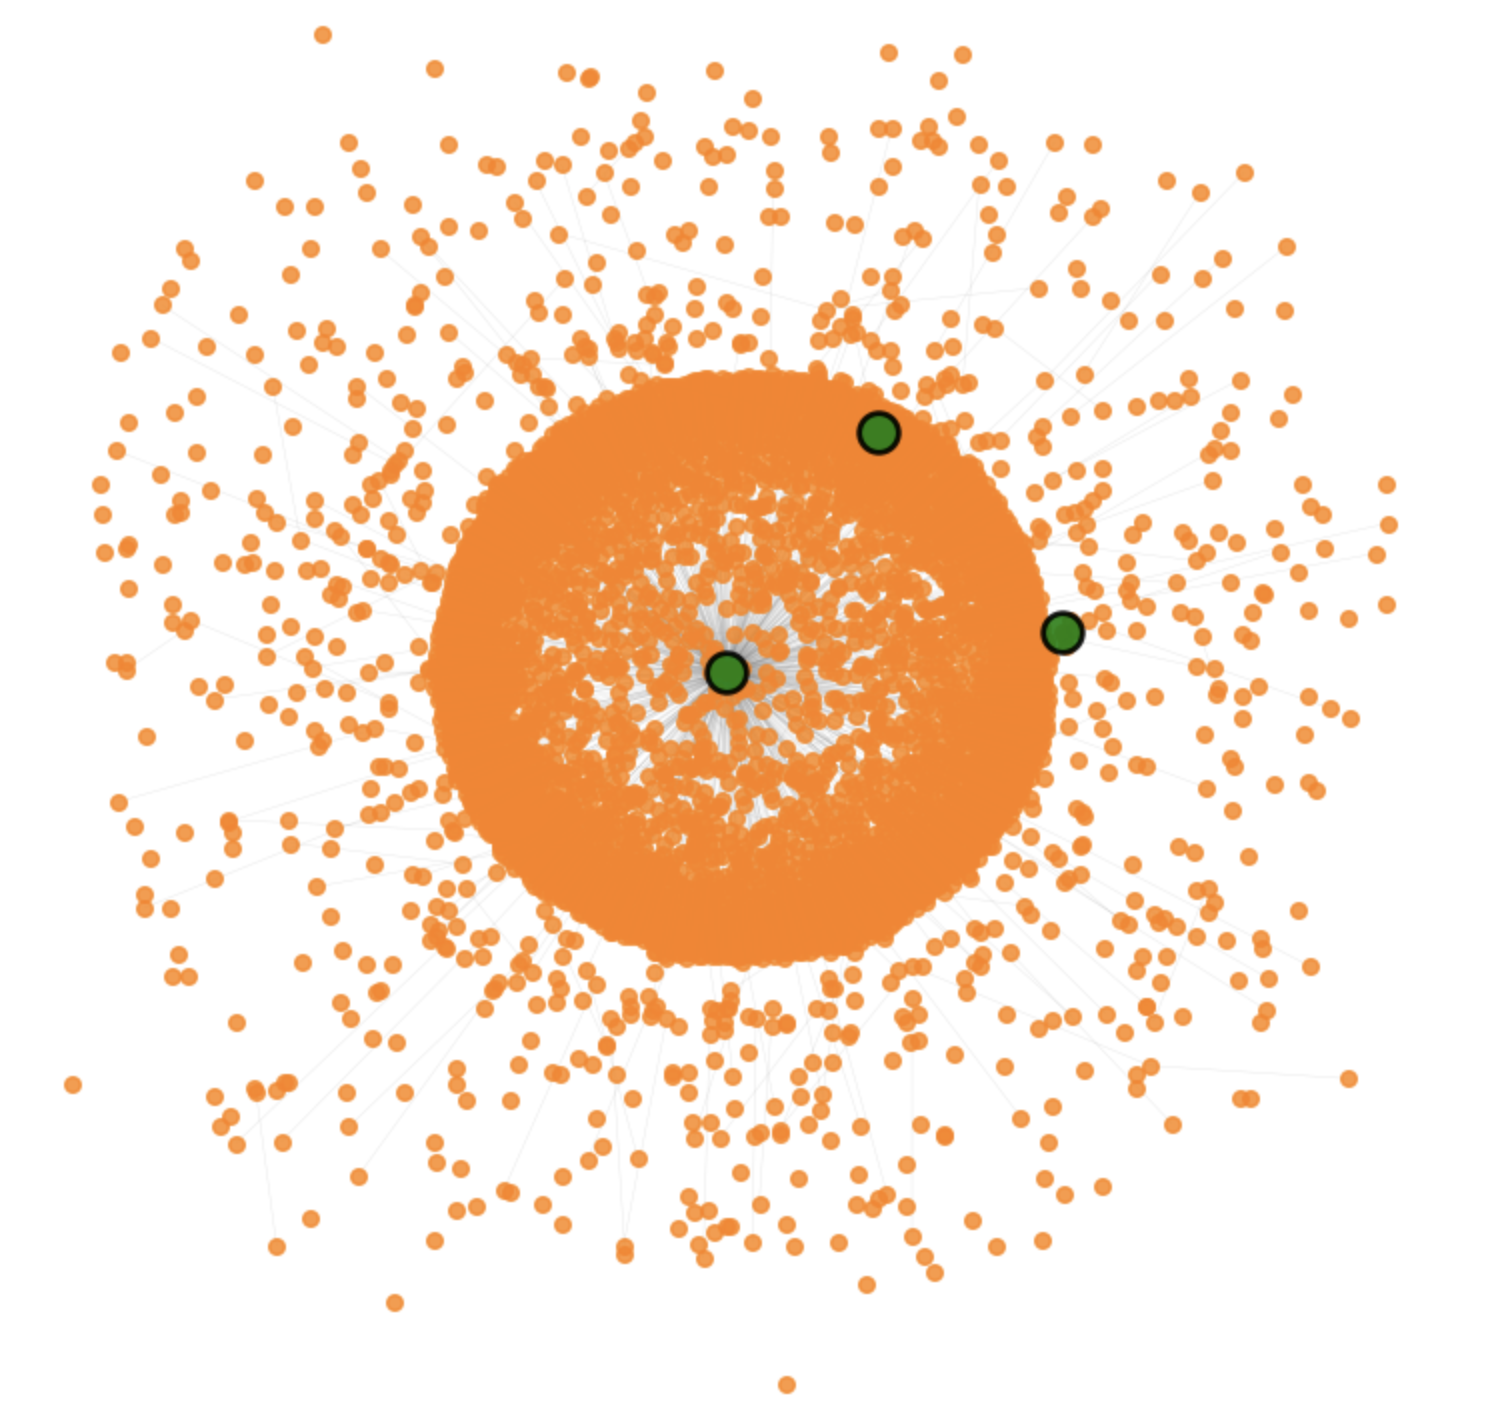
\includegraphics[width=\textwidth]{images/6.png}
	\end{center}
	\caption{Визуализация восьмого по величине сообщества (4 876 узлов) и трёх самых влиятельных узлов в нём (влияют на 80.6\% сообщества)}
	\label{img:6}
\end{figure}

\clearpage
